% =====================================================================
% Supplementary Information (reconstructed editable LaTeX source).
% Built with tectonic: `tectonic supplement.tex`
% =====================================================================
\documentclass[11pt]{article}
\usepackage[margin=1in]{geometry}
\usepackage{graphicx}
\usepackage{amsmath}
\usepackage{amssymb}
\usepackage{microtype}
\usepackage{setspace}
\usepackage[font=small,labelfont=bf]{caption}
\usepackage[hidelinks]{hyperref}

\graphicspath{{../figures/manuscript/}}

\newcommand{\Dstar}{\ensuremath{D^{*}}}

\setstretch{1.15}
\setlength{\parskip}{0.5em}
\setlength{\parindent}{0pt}

% Number supplementary figures as S1, S2, ...
\renewcommand{\thefigure}{S\arabic{figure}}

\begin{document}

\begin{center}
{\Large\bfseries Supplementary Information\par}
\vspace{0.6em}
{\itshape Calibration and Efficiency of Uncertainty Estimates in Intravoxel Incoherent Motion
Imaging\par}
\vspace{0.4em}
Avery Karlin, BA --- Columbia University (Applied Physics and Applied Mathematics) and
University of Colorado Boulder (Computer Science)
\end{center}

\vspace{1em}

\section*{Supplementary Methods}

\subsection*{S1. Architecture ablation (Masked Autoregressive Flow)}

To test whether the \Dstar{} pointwise overconfidence is specific to the neural spline flow,
the density estimator was replaced with a Masked Autoregressive Flow (5 MADE layers) while
holding the permutation-invariant embedding network, the BoxUniform prior, the
$\log_{10}$-SNR conditioning, and the training budget identical to the primary configuration.
The MAF was audited on the same dense CRLB benchmarking grid; for \Dstar{} across the SNR
10--100 grid, the claimed posterior SD and the achieved empirical SD (scatter of the
posterior mean across 50 noise realizations) were recorded and expressed as a ratio to the
CRLB floor. No out-of-distribution, acquisition-shift, or in-vivo evaluations were repeated
for the MAF.

\subsection*{S2. Dense-acquisition control}

To separate prior-reversion from the sparsity of the clinical acquisition, a second NPE was
trained and evaluated entirely on a dense 16-point b-scheme ($\{0, 10, 20, 30, 50, 75, 100,
150, 200, 300, 400, 500, 600, 700, 800, 1000\}$~s/mm$^2$) under the identical recipe to the
primary model (set representation, neural spline flow, 500,000-simulation budget, log-\Dstar{}
prior, matched seed). The dense model is in-distribution for its own scheme (not the
off-scheme evaluation of Figure 4C) and is audited against the correspondingly tighter dense
CRLB floor; it trained to convergence (169 epochs). Per-SNR median \Dstar{} SD-to-CRLB ratios
reproduce the main-text Figure 3 transform over the 512-point grid.

\subsection*{S3. Operationalized out-of-distribution gate}

The deployment-time gate was operationalized at the voxel level on the in-vivo brain dataset
(OSIPI TF2.4 IVIM-MRI Code Collection data, Zenodo doi:10.5281/zenodo.14605039;
$N \approx 2{,}000$ gray-matter voxels). This is the same gray-matter ROI and held-out-b
partition as the $N = 500$ held-out-b coverage check in main-text Figure 4B; the larger sample
is drawn here because a per-voxel ROC threshold requires more voxels than an aggregate coverage
curve, and the two are overlapping random draws from the same voxel pool rather than distinct
datasets. For each voxel two deployable scores were computed
from the fit b-values only: the reduced $\chi^2$ of the biexponential NLLS fit (a classical,
NPE-independent goodness-of-fit signal) and an NPE posterior-predictive self-consistency
residual. Each was scored against the held-out-b posterior-predictive miscalibration
(computed on a disjoint b-value set, so prediction is a genuine generalization test, not a
tautology) by ROC AUC and by calibration recovery as a function of retained fraction. The
recommended threshold is the ROC Youden point of the self-consistency gate.

\subsection*{S5. Prior-sensitivity ablation}

To test whether the below-floor \Dstar{} overconfidence depends on the prior, a second NPE was
trained under the identical setB recipe (set representation, neural spline flow,
500,000-simulation budget, matched seed, clinical-sparse b-scheme), changing only the \Dstar{}
prior from log-uniform to a tissue-informed truncated Normal on $\log_{10}(\Dstar)$ ($\mu =
\log_{10}(0.03)$, $\sigma = 0.30$~dex). It was audited against the same analytical CRLB grid
and the same per-SNR median-ratio transform as the primary model.

\subsection*{S6. Training-simulation-budget sweep}

To test whether the below-floor \Dstar{} overconfidence reflects an intrinsic property of the
amortized estimator or merely simulation starvation, the NPE was retrained at five
training-simulation budgets (50{,}000; 100{,}000; 250{,}000; 500{,}000; 1{,}000{,}000) with
everything else held fixed (set representation, neural spline flow, $\log_{10}(\Dstar{})$
prior, matched seed, clinical-sparse b-scheme), and each model was put through the identical
CRLB efficiency audit. Across the 20-fold budget range the per-SNR median \Dstar{} claimed
and achieved SD-to-CRLB ratios and the below-floor fraction were essentially flat (overall
\Dstar{} below-floor fraction 0.69--0.70; claimed ratio at SNR 10 in 0.077--0.084; achieved
ratio at SNR 10 in 0.016--0.019). The below-floor overconfidence is therefore not a
small-sample/training-starvation artifact.

\subsection*{S7. In-silico parameter-calibration control and model criticism}

To separate posterior-width overconfidence from forward-model misfit --- which the in-vivo
signal-domain check cannot disentangle --- the trained NPE was evaluated on simulated voxels
with \emph{known} parameters (4{,}000 draws from the prior; SNR log-uniform 8--100) on its
own training acquisition with the correct forward model. Empirical parameter coverage was the
fraction of voxels whose true $[D, \Dstar{}, f]$ fell within the central $L$-level posterior
interval, computed overall and stratified by SNR and by perfusion fraction. With the correct
forward model and on the training acquisition, coverage was near-nominal (0.93--0.94 at
nominal 0.95) and remained near-nominal across strata, establishing that the in-distribution
parameter posterior is Bayesian-calibrated and that the pointwise overconfidence reported in
the main text is an information-floor (efficiency) and signal-prediction phenomenon rather
than an in-distribution parameter-coverage failure. As a robust-NPE-style (RNPE) model
criticism, each in-vivo voxel's posterior-predictive self-consistency residual was compared to
an SNR-matched 95th-percentile null built from the well-specified simulation; the flagged
fraction (12.8\%, versus a 5\% well-specified baseline) is reported as a misspecification
diagnostic. The control uses no in-vivo parameter ground truth; a definitive in-vivo
parameter-recovery test would require phantom or repeated-acquisition data and remains open.
This control was a one-time analysis and was not part of the per-SNR median-ratio transform.

\section*{Supplementary Figures}

\begin{figure}[htbp]
\centering
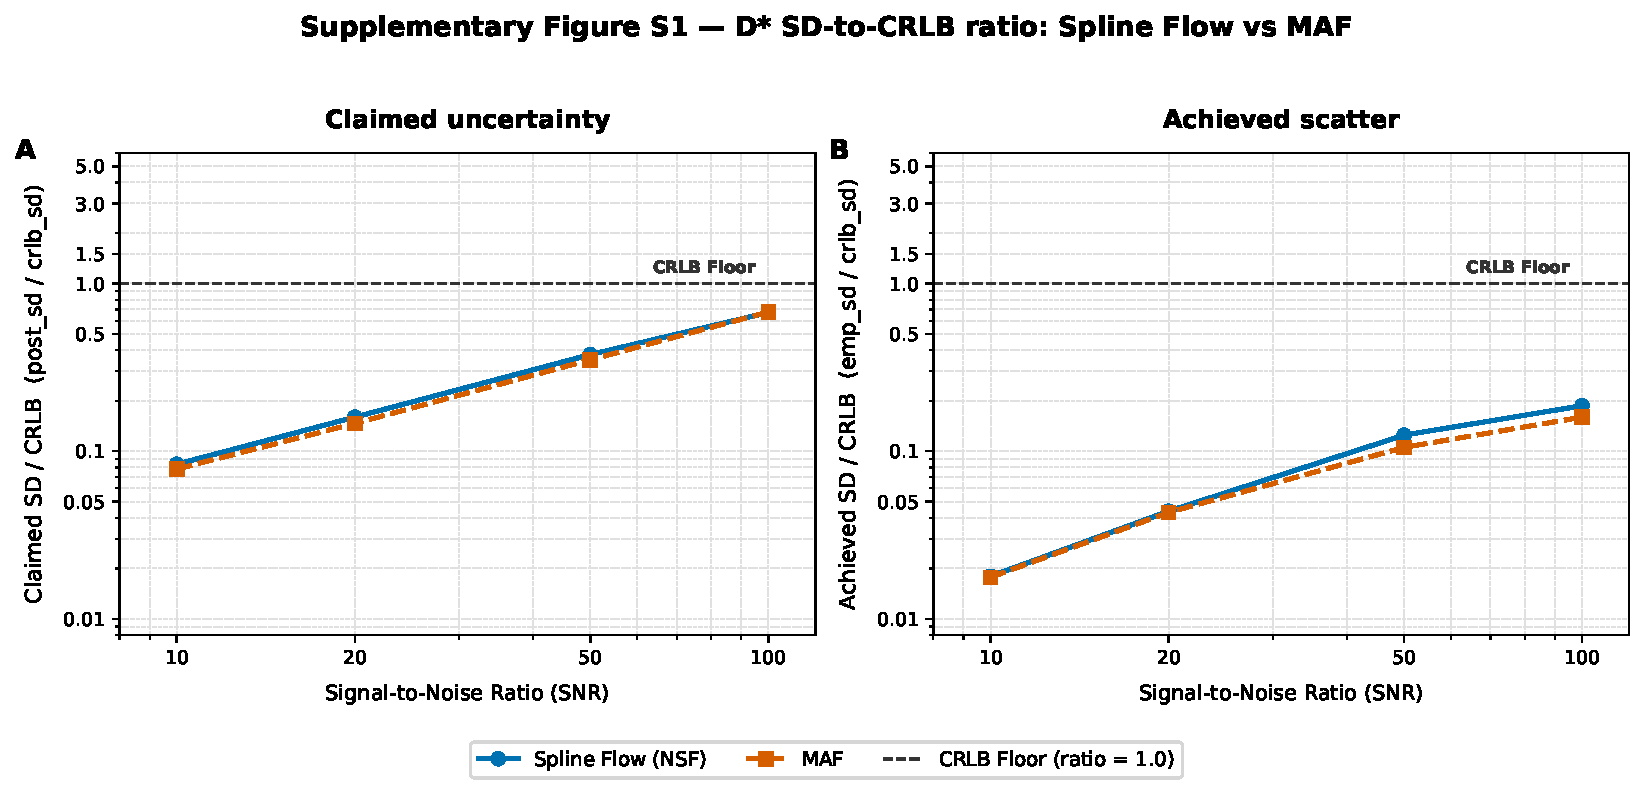
\includegraphics[width=\textwidth]{figS1_maf_ablation.pdf}
\caption{Architecture ablation. \Dstar{} SD-to-CRLB ratio versus SNR for the neural spline
flow and the Masked Autoregressive Flow (per-SNR medians). (A) Claimed posterior SD ratio;
(B) achieved empirical SD ratio. Both architectures sit well below the CRLB floor (ratio =
1.0) across SNR, with the MAF reproducing the same below-floor overconfidence (claimed ratio
within 6--8\% of the spline flow at SNR 10--50 and within 1\% at SNR 100; achieved ratio
within $\sim$15\% across SNR), indicating the \Dstar{} overconfidence is architecture-agnostic
rather than an artifact of the spline-flow density estimator.}
\end{figure}

\begin{figure}[htbp]
\centering
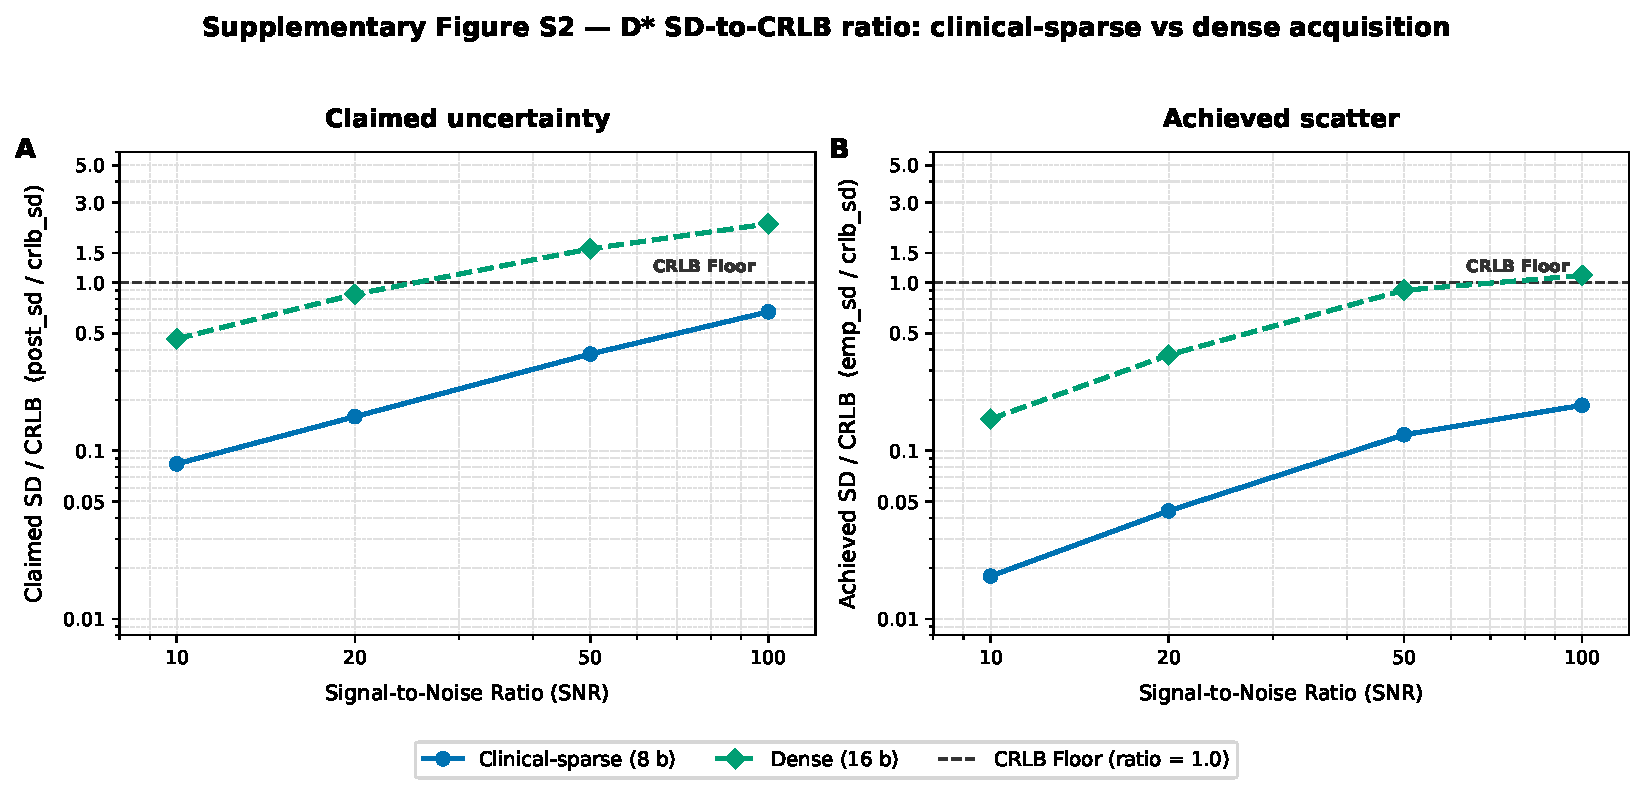
\includegraphics[width=\textwidth]{figS2_dense_acquisition.pdf}
\caption{Dense-acquisition control. \Dstar{} SD-to-CRLB ratio versus SNR for the
clinical-sparse (8 b) and dense (16 b) NPEs, each audited against its own CRLB floor. (A)
Claimed posterior SD ratio; (B) achieved empirical SD ratio. The dense model's claimed \Dstar{}
uncertainty stays below the floor through the clinical SNR regime (ratio 0.46 at SNR 10, 0.85
at SNR 20; 41\% of grid points overconfident overall vs 69\% clinical-sparse), crossing to
inefficiency only at high SNR. The below-floor overconfidence is mitigated but not eliminated
by denser sampling.}
\end{figure}

\begin{figure}[htbp]
\centering
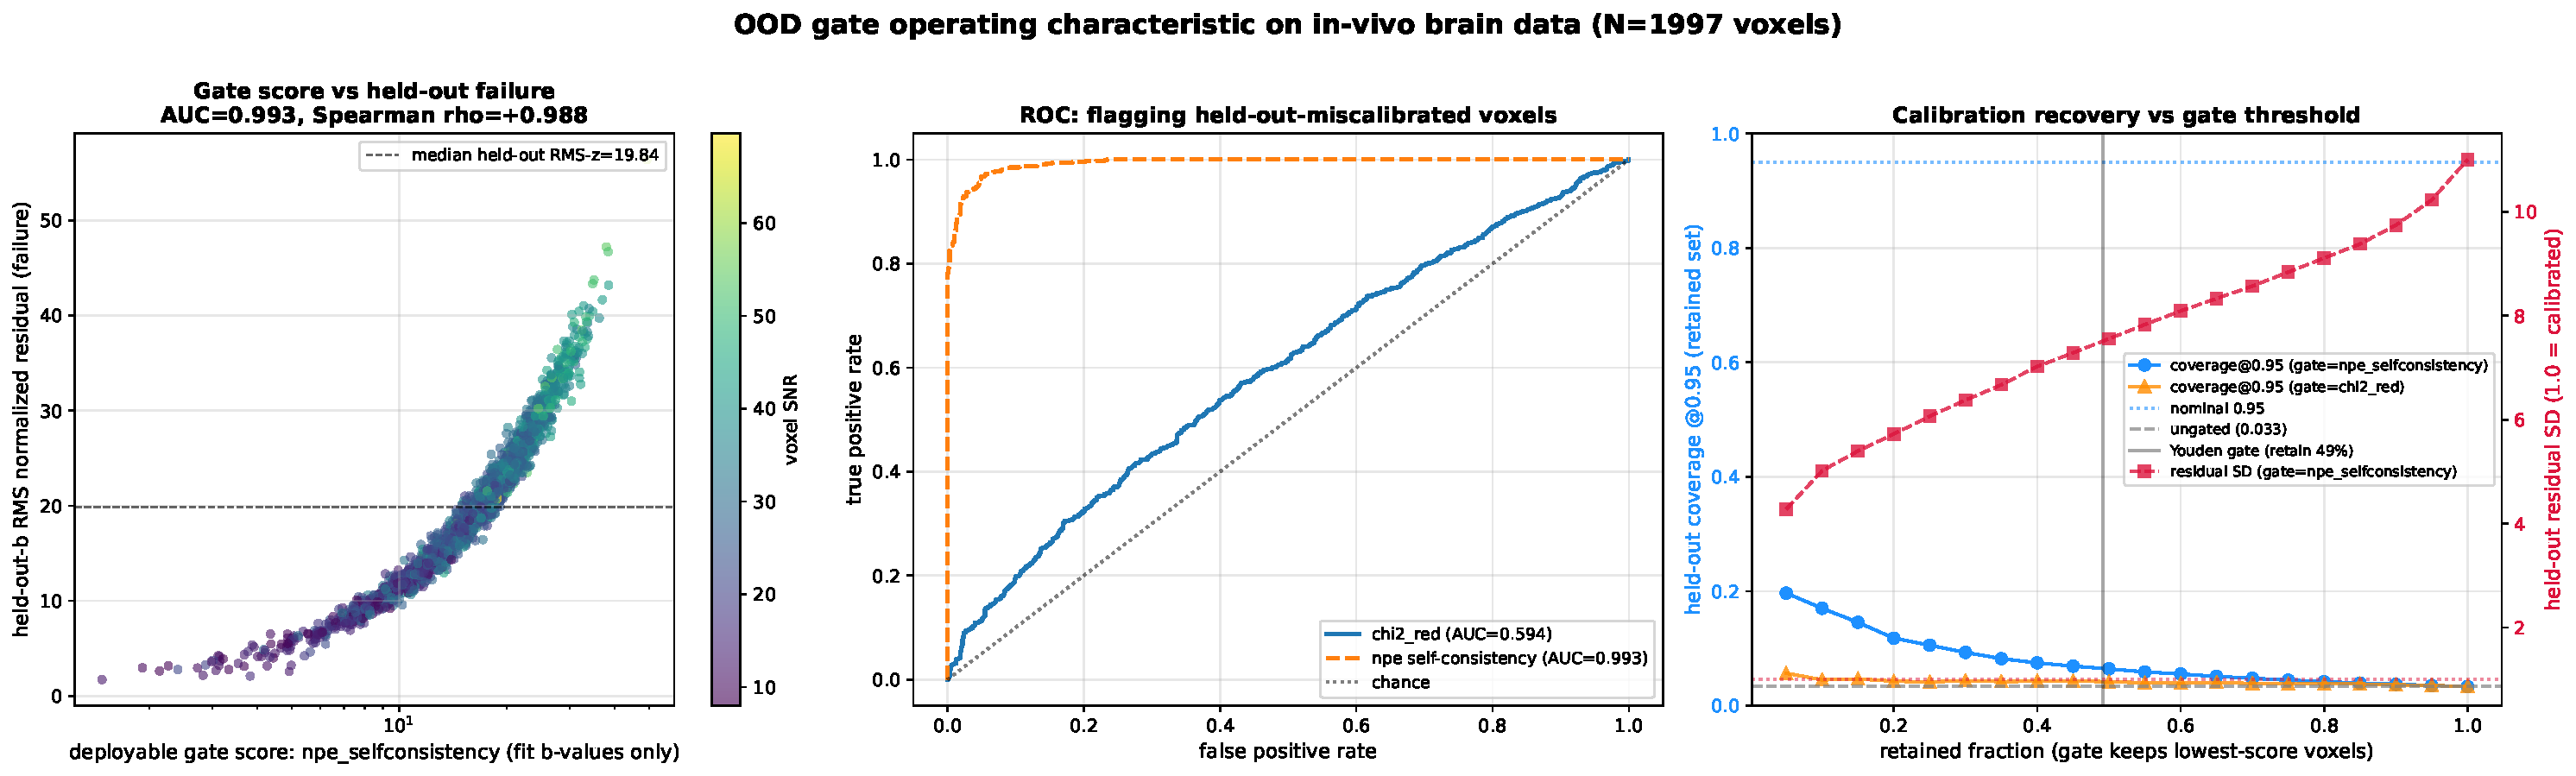
\includegraphics[width=\textwidth]{figS3_ood_gating.pdf}
\caption{Deployable out-of-distribution gate on the in-vivo brain dataset. (A) Held-out-b
coverage and (B) held-out normalized-residual SD as the retained voxel fraction is tightened,
for the NPE posterior-predictive self-consistency gate (AUC 0.99 against the unobservable
held-out miscalibration) versus a classical biexponential goodness-of-fit $\chi^2$ gate (AUC
0.59). The self-consistency gate monotonically recovers coverage ($0.03 \to 0.20$) and reduces
residual SD ($11.0 \to 4.3$); the $\chi^2$ gate does not, confirming the overconfidence is
intrinsic to the estimator rather than model-misfit. Marked point: ROC Youden threshold
(self-consistency $\le 16.7$, TPR 0.97 / FPR 0.05, 49\% retained).}
\end{figure}

\begin{figure}[htbp]
\centering
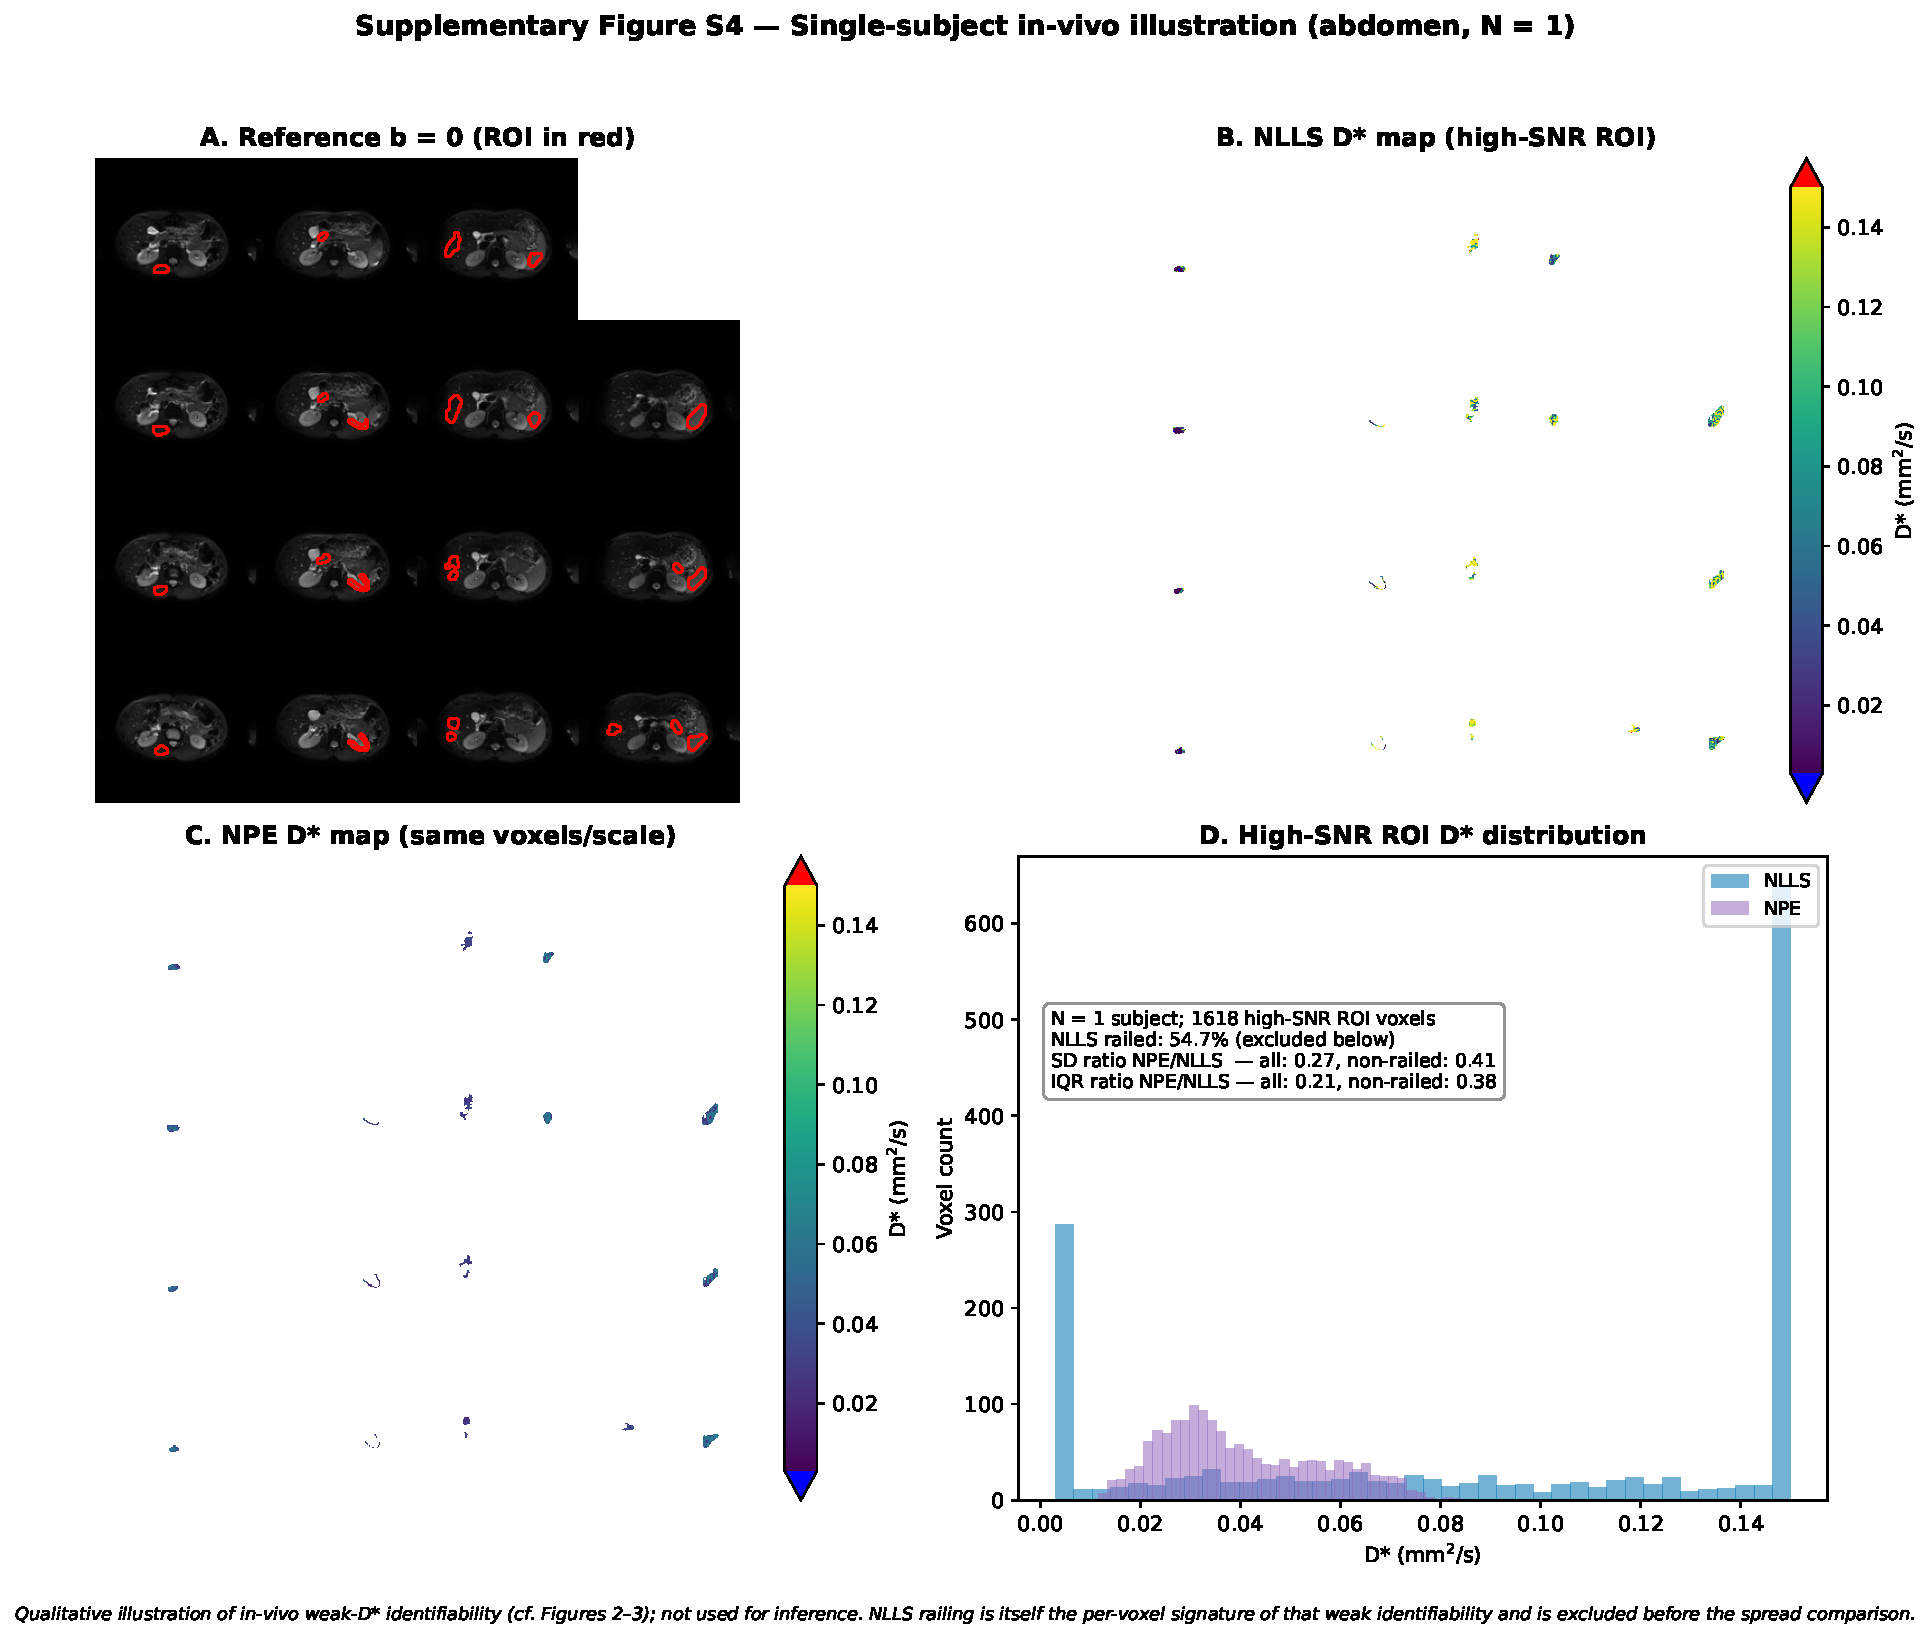
\includegraphics[width=\textwidth]{figS4_invivo_illustration.pdf}
\caption{Single-subject in-vivo illustration (abdomen, $N = 1$). NPE and biexponential-NLLS
\Dstar{} maps for one open IVIM abdominal acquisition from the same collection (OSIPI TF2.4
IVIM-MRI Code Collection data, Zenodo doi:10.5281/zenodo.14605039). In 54.7\% of high-SNR ROI
voxels the NLLS \Dstar{}
estimate is boundary-railed, which is the per-voxel signature of the weak \Dstar{}
identifiability characterised in simulation (Figures 2--3). The \Dstar{} spread ratio
(NPE$/$NLLS) is reported both ways to make the inclusion policy explicit: railed-included
(all 1{,}618 voxels) SD ratio 0.27 / IQR ratio 0.21, and railed-excluded (733 non-railed
voxels) SD ratio 0.41 / IQR ratio 0.38. The railed-excluded values (the OLD reported pair)
are the more conservative for the overconfidence narrative, because the boundary-pinned NLLS
values are degenerate point masses that inflate the NLLS spread and thus shrink the ratio when
included; we therefore quote the non-railed ratio as primary but report both. The case is
shown as a qualitative illustration of that mechanism in
vivo and is not used to support any quantitative claim; $N = 1$ precludes population inference.}
\end{figure}

\begin{figure}[htbp]
\centering
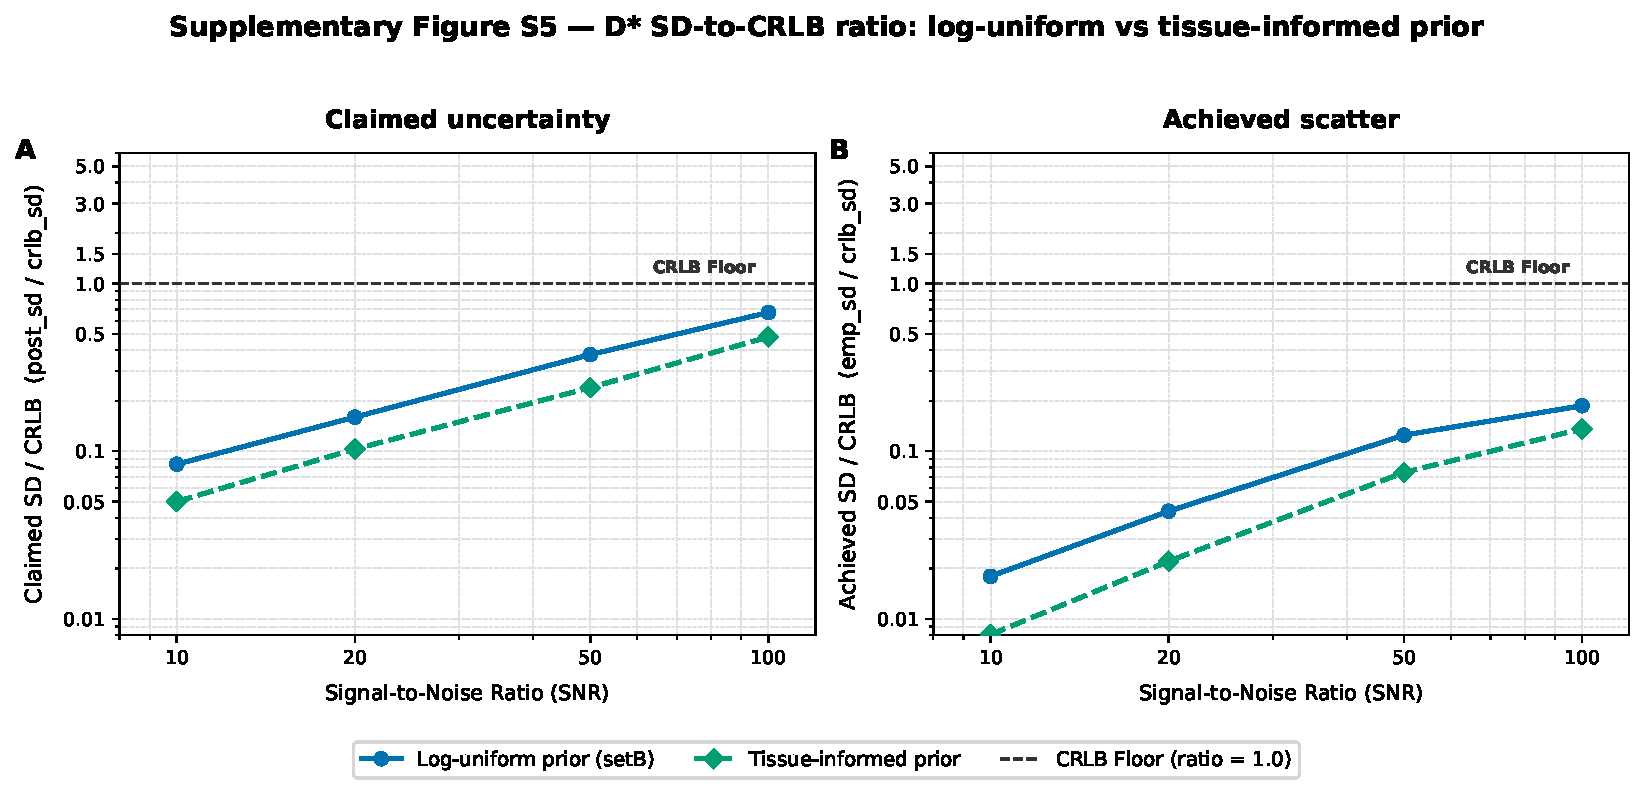
\includegraphics[width=\textwidth]{figS5_prior_ablation.pdf}
\caption{Prior-sensitivity ablation. Fraction of \Dstar{} grid points with claimed SD below
the CRLB floor, by SNR, for the primary log-uniform prior versus a tissue-informed
truncated-Normal \Dstar{} prior (otherwise identical recipe). The below-floor overconfidence
persists, and is slightly higher, under the tissue prior at every SNR (overall 76.3\% versus
69.5\%). An informative prior legitimately permits posterior width below the prior-free CRLB,
so the discriminating evidence is the persistence under the uninformative log-uniform prior
and in both claimed and achieved SD, indicating the overconfidence is intrinsic to the
amortized estimator rather than prior-reversion.}
\end{figure}

\begin{figure}[htbp]
\centering
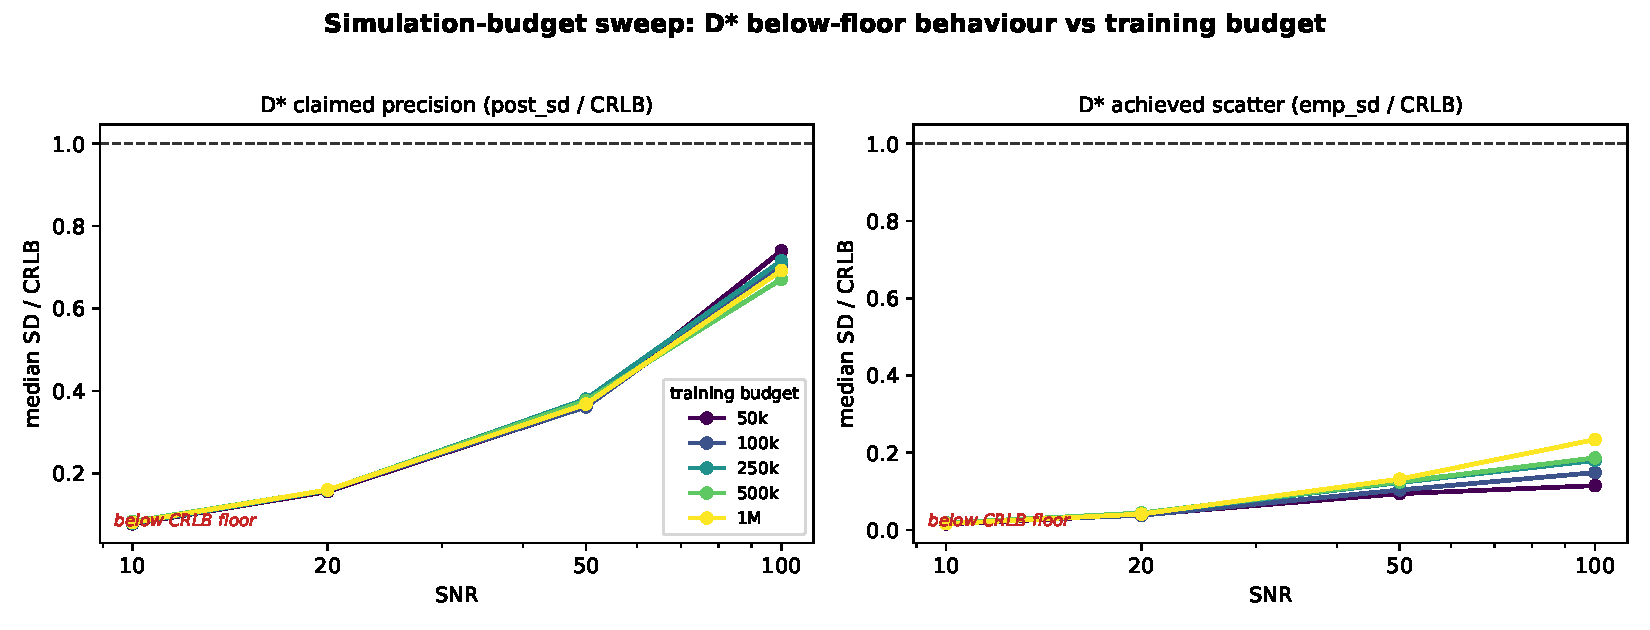
\includegraphics[width=\textwidth]{figS6_budget_sweep.pdf}
\caption{Training-simulation-budget sweep. Per-SNR median \Dstar{} SD-to-CRLB ratio versus SNR
for NPEs trained at budgets of 50k, 100k, 250k, 500k, and 1M simulations, everything else held
fixed. (A) Claimed posterior SD ratio; (B) achieved empirical SD ratio. The curves are nearly
coincident: the below-floor \Dstar{} overconfidence is invariant across the 20-fold budget
range (overall below-floor fraction $\approx$0.69 at every budget), so it is an intrinsic
property of the amortized estimator under weak identifiability, not an artifact of
insufficient training simulations.}
\end{figure}

\end{document}
